\subsection{FISTA}
A possible solver is \fista, first introduced in~\cite{fista}.
The discussion of \fista\ follows~\cite{fista}, the description of
the proximal operators follows~\cite{proxsurvey}.
\fista\ is able to minimize functions that can be expressed as a sum of a convex,
smooth function \(f\) and another convex, possibly non-smooth function \(g\): 
\begin{equation}\label{eq:composite-goal}
F(\bm{\alpha}) = f(\bm{\alpha}) + g(\bm{\alpha}). 
\end{equation}

It is required that the function \(f(\bm{\alpha})\) has a Lipschitz-continuous gradient. 
This means that the following condition has to be valid for all possible
vectors \(\bm{x}\) and \(\bm{y}\) for some constants \(L\):
\begin{equation}   \label{eq:lipschitz}
 \Vert \nabla f(\bm{x}) - \nabla f(\bm{y}) \Vert \leq L \Vert \bm{x} - \bm{y} \Vert.
\end{equation}
We call the smallest possible value of \(L\) the Lipschitz constant.

In our case we set \(f\) to
\begin{equation*}
 f(\bm{\alpha}) = \frac{1}{2} \left\Vert  \bm{\Phi} \bm{\alpha} - \bm{y}   \right\Vert_2^2.
\end{equation*}
The gradient of \(f\) is then given by
\begin{equation*}
  \nabla f(\bm{\alpha}) = \bm{\Phi}^\intercal \left(\bm{\Phi} \bm{\alpha} - \bm{y} \right).
\end{equation*}
The Lipschitz constant for the gradient of \(f\) is
\begin{equation}
  \label{eq:lipf}
  L_{\nabla f} = {\left[\sigma_{\max} \left(\bm{\Phi}\right)\right]}^2,
\end{equation}
where \(\sigma_{\max} \) corresponds to the maximum singular value.

Additionally we set \(g\) to
\begin{equation*}
  g(\bm{\alpha}, \lambda) = \mathcal{S} \left( \bm{\alpha}, \lambda \right).
\end{equation*}
We now need to define a function that minimizes \(g\).
A unique minimizer for a scaled convex function \(\lambda g\) is given by the so called
proximal operator 
\begin{equation}
  \label{eq:proximal}
  \prox[\(g\)]{\bm{\alpha}}{\lambda}= \argmin_{\bm{x}} \left\{ g (\bm{x}) + (1/ (2 \lambda)) \Vert \bm{x} - \bm{\alpha} \Vert_2^2 \right\}.
\end{equation}
In the most general case this would imply the need to solve a convex
optimization problem.
We can find closed form solutions for many functions.
If we do not use a regularization operator, we can use the function \(g = 0\) as
our smoothness term.
In this case the proximal operator is trivial, it is given by the identity
function
\begin{equation*}
 \prox[id]{\bm{\alpha}}{\lambda} = \alpha.
\end{equation*}

We define a quadratic approximation of \(f (\bm{\alpha}) + g (\bm{\alpha})\) for a given \(L > 0\)
at a point \(\bm{y}\) as
\begin{equation}\label{eq:goal-approx}
  Q_{L} = f(\bm{y}) + \left< \bm{\alpha} - \bm{y}, \nabla f(\bm{y}) \right> + \frac{L}{2} \Vert \bm{\alpha} - \bm{y} \Vert_2^2 + g(\bm{\alpha}),
\end{equation}
where the angle brackets \( \left< \bm{x}, \bm{y} \right> = \bm{y}^\intercal \bm{x} \) represent the inner product.
The minimizer for this approximation is then given as the fixed-point equation
\begin{align}\label{eq:step}
\pi_L(\bm{\alpha}^*, \lambda) &= \prox[\(g\)]{\bm{\alpha^*} - L^{-1} \nabla f (\bm{\alpha^*})}{\lambda L^{-1} } \nonumber\\
       &= \prox[\(g\)]{\bm{\alpha^*} - L^{-1} \bm{\Phi}^\intercal \left(\bm{\Phi} \bm{\alpha^*} - \bm{y} \right)}
         {\lambda L^{-1}},
\end{align}
where \(\bm{\alpha}^*\) denotes the optimal solution and \(L\) is the Lipschitz
constant of \(\nabla f\) given by \autoref{eq:lipf}.
In this equation \(L\) is used to determine the optimal stepsize.

\begin{algorithm}
 \caption{Iterative Shrinkage Tresholding Algorithm}\label{alg:ista} 
 \begin{algorithmic}[1]
   \Require{Lipschitz constant \(L\) of \(\nabla f\), regularization parameter \(\lambda\)}
    \Statex
    \Function{Ista}{$L, \bm{\alpha}$} \Comment{\(\bm{\alpha}\) is an initial guess}
      \While{not converged}
        \Let{$\bm{\alpha}$}{\( \pi_L \left( \bm{\alpha}, \lambda \right) \)}
      \EndWhile
     \State \Return{\(\bm{\alpha}\)}
    \EndFunction
\end{algorithmic}
\end{algorithm}

These preliminary definitions are enough to define the simple iterative
algorithm called \ista as seen in \autoref{alg:ista}.
For our trivial function \(g\) this iterative scheme is identical to the standard gradient descent algorithm.
This optimization method always converges to the global maximum, but only
linearly. The full proof of this behavior is given in~\cite{fista}.

So far we have only seen the proximal operator of a very simple function.
There are also such operators for more complicated regularization methods.
We need the following closed form solutions:
\begin{align}
\label{eq:prox-lasso}
\text{(Lasso)} \quad &&
\left( \prox[\(\Vert \cdot \Vert_1\)]{\bm{\alpha}}{\lambda} \right)_i &= \left(\alpha_i - \lambda \right)_+ - \left( -\alpha_i - \lambda \right)_+, \\
\text{(Ridge)} \quad &&
 \prox[\(\Vert \cdot \Vert_2\)]{\bm{\alpha}}{\lambda} &= \left[ \left(1 - \lambda \right) \left(  \Vert \bm{\alpha } \Vert_2\right)^{-1} \right]_+,
\end{align}
where \( \left( x \right)_+ = \max(x, 0) \) denotes the positive part of \(x\).
The derivations are omitted for the sake of brevity, the interested reader is referred to the survey paper~\cite{proxsurvey}.
We observe, that by setting the regularization parameter \(\lambda\) equal to zero, we recover, again, the gradient minimization method.

These proximal operators can be used to define a minimizer for a non-smooth
function \(g\).
For example, combining~\autoref{eq:step} with the proximal operator for the
Lasso functional \(g(\bm{\alpha}) = \lambda \Vert \bm{\alpha} \Vert_1\) given by~\autoref{eq:prox-lasso} results in
the minimizer
\begin{equation*}
  \pi_{L \Vert \cdot \Vert_1}(\bm{\alpha^*} ,\lambda)
  = {\left[ \left(\bm{\alpha^*} - L^{-1} \nabla f (\bm{\alpha^*}) \right) - \lambda L^{-1} \right]}_+ -
    {\left[ -\left(\bm{\alpha^*} - L^{-1} \nabla f (\bm{\alpha^*}) \right) - \lambda L^{-1} \right]}_+,
\end{equation*}
again given as a fixed-point iteration.
In this equation the function \( \left( x \right)_+ \) is applied element-wise on its input vector.

This optimization method always converges to the global maximum, but only
linearly. The full proof of this behavior is given in~\cite{fista}.
To overcome this problem, Beck and Teboulle combined the \ista algorithm with the accelerated gradient descent algorithm discovered by Nesterov. 
This augmented algorithm archives quadratic convergence and is called \fista.
Each step of \fista\ evaluates the gradient and the proximal operator once, just as \ista does.
This means that the accelerated algorithm has a comparable cost for each iteration.

Another problem with \autoref{alg:ista} is its dependence on the Lipschitz constant of
\(\nabla f\) to determine the optimal stepsize.
For our choice of \(f\), the best constant \(L\) is given by~\autoref{eq:lipf}.
To avoid this expensive calculation, we use a backtracking line search to
determine a suitable stepsize.
In this line search procedure we use \autoref{eq:goal-approx} as an upper bound for \autoref{eq:composite-goal}.
It is then straightforward to derive \autoref{alg:linesearch}.

\begin{algorithm}[H]
 \caption{Linesearch}\label{alg:linesearch}
 \begin{algorithmic}[1]
  \Require{\(L > 0, \eta > 1, \bm{\alpha}\)} 
  \Statex
  \Function{Linesearch}{$\bm{\alpha}, L$}
    \Let{\(i\)}{\(0\)}
    \Do
      \Let{L}{\(\eta^i L\)}
      \Let{prox}{\(\pi (\bm{\alpha}, L)\)}
      \Let{\(i\)}{\(i + 1\)}
    \doWhile{$F(\text{prox}) < Q_L(\text{prox}, \bm{\alpha})$}
    \State \Return{prox and \(L\)} \Comment{Also return prox to avoid duplicate calculations.}
  \EndFunction
 \end{algorithmic}
\end{algorithm}

We need to evaluate the line search once for each iteration step.
This line search always finds a suitable approximation for \(L\) given correct
starting values.
It is possible that this procedure finds a non-optimal stepsize, i.e.~a
stepsize that is smaller than the optimal one.
This is not a problem in practice, our optimization procedure still converges,
but slower. 

Using these definitions we can finally present the optimal optimization
algorithm, shown by \autoref{alg:fista}.

\marginline{The same line search can be used to determine the stepsize for \ista.}
It is of course possible to use a constant stepsize like in \autoref{alg:ista}.
To do this, start the line search with the minimal value of \(L\).
The linesearch then terminates after the first iteration and is therefore as fast as calculating \autoref{eq:step}.
A comparison of the practical speed of \ista and \fista with constant stepsize can be seen in~\autoref{fig:fista-convergence}.
\begin{figure}[T]
  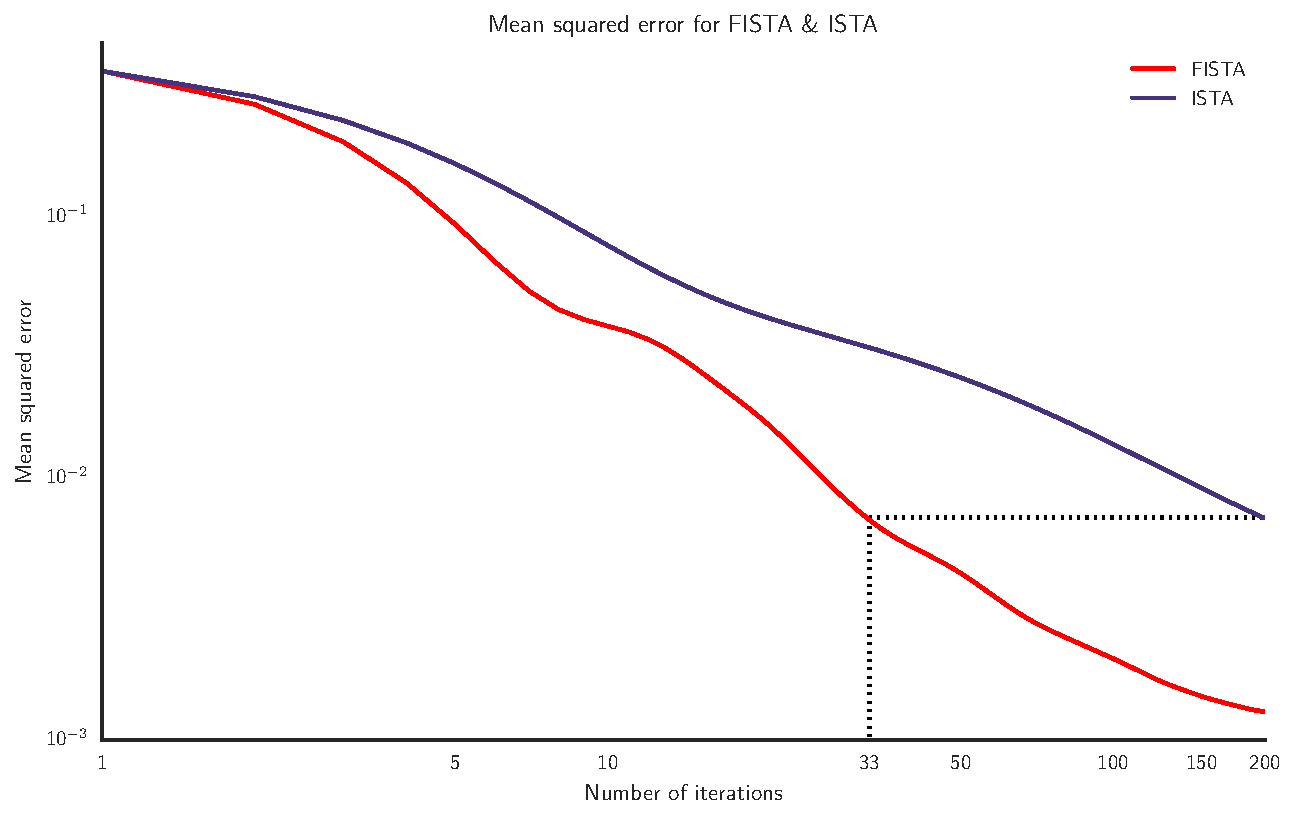
\includegraphics[scale=0.6]{fista}
  \caption{Comparison of \fista and \ista, both with constant stepsize.
    The figure shows the training mean squared error for the first 1000 iterations with \(\lambda = 0.001\) for the training set of the concrete data set.}\label{fig:fista-convergence}
\end{figure}

\begin{algorithm}[H]
 \caption{Fast Iterative Shrinkage Tresholding Algorithm} \label{alg:fista} 
 \begin{algorithmic}[1]
   \Require{Initial guess for Lipschitz constant \(L\) of \(\nabla f\), regularization parameter \(\lambda\)}
    \Statex
    \Function{Fista}{$L, \bm{\alpha}$} \Comment{\(\bm{\alpha}\) is an initial
      guess for \(\alpha^*\).}
      \Let{\(\bm{y}\)}{\(\bm{\alpha}\)}
      \Let{\(t\)}{\(1\)}
      \While{not converged}
        \Let{$\bm{\alpha}, L$}{\Call{Linesearch}{$ \bm{y}, L$ }} \Comment{Linesearch returns \(\pi_L (\bm{y})\) and the used L.}
        \Let{\(t_\text{before}\)}{\(t\)}
        \Let{\(t\)}{\(\nicefrac{1}{2} (1 + \sqrt{1+4t^2}) \)}
        \Let{\(\bm{y}\)}{\(\bm{\alpha} + \left( t_\text{before} -1 \right) t^{-1} 
                    \left(\bm{\alpha} - \bm{\alpha}_{\text{before}} \right)\)}
      \EndWhile
     \State \Return{\(\bm{\alpha}\)}
    \EndFunction
\end{algorithmic}
\end{algorithm}

%%% Local Variables:
%%% mode: latex
%%% TeX-master: "../main"
%%% End:
